%%
%% This is file `sample-xelatex.tex',
%% generated with the docstrip utility.
%%
%% The original source files were:
%%
%% samples.dtx  (with options: `sigconf')
%% 
%% IMPORTANT NOTICE:
%% 
%% For the copyright see the source file.
%% 
%% Any modified versions of this file must be renamed
%% with new filenames distinct from sample-xelatex.tex.
%% 
%% For distribution of the original source see the terms
%% for copying and modification in the file samples.dtx.
%% 
%% This generated file may be distributed as long as the
%% original source files, as listed above, are part of the
%% same distribution. (The sources need not necessarily be
%% in the same archive or directory.)
%%
%% The first command in your LaTeX source must be the \documentclass command.
\documentclass[sigconf]{acmart}

%%
%% \BibTeX command to typeset BibTeX logo in the docs
\AtBeginDocument{%
  \providecommand\BibTeX{{%
    \normalfont B\kern-0.5em{\scshape i\kern-0.25em b}\kern-0.8em\TeX}}}

%% Rights management information.  This information is sent to you
%% when you complete the rights form.  These commands have SAMPLE
%% values in them; it is your responsibility as an author to replace
%% the commands and values with those provided to you when you
%% complete the rights form.
\setcopyright{acmcopyright}
\copyrightyear{2019}
\acmYear{2019}
\acmDOI{10.1145/1122445.1122456}

%% These commands are for a PROCEEDINGS abstract or paper.
\acmConference[Woodstock '18]{Woodstock '18: ACM Symposium on Neural
  Gaze Detection}{June 03--05, 2018}{Woodstock, NY}
\acmBooktitle{Woodstock '18: ACM Symposium on Neural Gaze Detection,
  June 03--05, 2018, Woodstock, NY}
\acmPrice{15.00}
\acmISBN{978-1-4503-9999-9/18/06}


%%
%% Submission ID.
%% Use this when submitting an article to a sponsored event. You'll
%% receive a unique submission ID from the organizers
%% of the event, and this ID should be used as the parameter to this command.
%%\acmSubmissionID{123-A56-BU3}

%%
%% The majority of ACM publications use numbered citations and
%% references.  The command \citestyle{authoryear} switches to the
%% "author year" style.
%%
%% If you are preparing content for an event
%% sponsored by ACM SIGGRAPH, you must use the "author year" style of
%% citations and references.
%% Uncommenting
%% the next command will enable that style.
%%\citestyle{acmauthoryear}

%%
%% end of the preamble, start of the body of the document source.
\usepackage{listings}
\usepackage{color}
\pagecolor{white}
\definecolor{dkgreen}{rgb}{0,0.6,0}
\definecolor{gray}{rgb}{0.5,0.5,0.5}
\definecolor{mauve}{rgb}{0.58,0,0.82}

\lstset{frame=tb,
  language=c++,
  aboveskip=3mm,
  belowskip=3mm,
  showstringspaces=false,
  columns=flexible,
  basicstyle={\small\ttfamily},
  numbers=none,
  numberstyle=\tiny\color{gray},
  keywordstyle=\color{blue},
  commentstyle=\color{dkgreen},
  stringstyle=\color{mauve},
  breaklines=true,
  breakatwhitespace=true,
  tabsize=3
}


\begin{document}

%%
%% The "title" command has an optional parameter,
%% allowing the author to define a "short title" to be used in page headers.
\title{Compression Point to Point Traffic Control}

%%
%% The "author" command and its associated commands are used to define
%% the authors and their affiliations.
%% Of note is the shared affiliation of the first two authors, and the
%% "authornote" and "authornotemark" commands
%% used to denote shared contribution to the research.
\author{Rozita Teymourzadeh}
\orcid{0000-0002-4620-7790}
\authornotemark[1]
\affiliation{%
  \institution{University of San Francisco}
  \city{San Francisco}
  \state{California}
  \postcode{94117}
}
\email{rteymourzadeh@usfca.edu}

\author{Ramona Carmen Stoica}
\orcid{0000-0002-4620-7790}
\authornotemark[2]
\affiliation{%
  \institution{University of San Francisco}
  \city{San Francisco}
  \state{California}
  \postcode{94117}
}
\email{rstoica@usfca.edu}

\author{Vahab Pournaghshband}
\orcid{0000-0002-4620-7790}
\authornotemark[3]
\affiliation{%
  \institution{University of San Francisco}
  \city{San Francisco}
  \state{California}
  \postcode{94117}
}
\email{vpournaghshband@usfca.edu}

%%
%% By default, the full list of authors will be used in the page
%% headers. Often, this list is too long, and will overlap
%% other information printed in the page headers. This command allows
%% the author to define a more concise list
%% of authors' names for this purpose.
\renewcommand{\shortauthors}{Trovato and Tobin, et al.}

%%
%% The abstract is a short summary of the work to be presented in the
%% article.
\begin{abstract}
Network traffic is an important issue raised by the network that refers to 
the amount of data moving across a network at the given point of time. 
A capsuled network data called packet is the main component for the 
traffic measurement and the network traffic shows a significant potential
for the researchers to find a solution on the high speed communication 
system \cite{campbell1974portable}\cite{bertsekas1987chapter}\cite{deng2012online}.  Several research works were conducted to transfer packets 
in high speed rate possibles and yet it is a challenging task.  In this research project, implementation of a network level compression link is considered. A network application to detect whether network compression is presented implemented. To validate the functionality, simulated compression link is designed and presented. In this research 
work, the focus was taken on the data compression approach to fully utilize 
the network when point to point network is a bottle neck. The design defined 
under under Microsoft  point to point protocol standard and network simulation 
(NS-3) environment were used for system design and implementation. 
A comprehensive data analysis and evaluation were conducted to observe 
network efficiency when compression is activated 
\end{abstract}

%%
%% The code below is generated by the tool at http://dl.acm.org/ccs.cfm.
%% Please copy and paste the code instead of the example below.
%%
\begin{CCSXML}
<ccs2012>
 <concept>
  <concept_id>10010520.10010553.10010562</concept_id>
  <concept_desc>Computer systems organization~Embedded systems</concept_desc>
  <concept_significance>500</concept_significance>
 </concept>
 <concept>
  <concept_id>10010520.10010575.10010755</concept_id>
  <concept_desc>Computer systems organization~Redundancy</concept_desc>
  <concept_significance>300</concept_significance>
 </concept>
 <concept>
  <concept_id>10010520.10010553.10010554</concept_id>
  <concept_desc>Computer systems organization~Robotics</concept_desc>
  <concept_significance>100</concept_significance>
 </concept>
 <concept>
  <concept_id>10003033.10003083.10003095</concept_id>
  <concept_desc>Networks~Network reliability</concept_desc>
  <concept_significance>100</concept_significance>
 </concept>
</ccs2012>
\end{CCSXML}

\ccsdesc[500]{Computer systems organization~Embedded systems}
\ccsdesc[300]{Computer systems organization~Redundancy}
\ccsdesc{Computer systems organization~Robotics}
\ccsdesc[100]{Networks~Network reliability}

%%
%% Keywords. The author(s) should pick words that accurately describe
%% the work being presented. Separate the keywords with commas.
\keywords{UDP, network traffic, point to point, packet, compression, zLib}

%% A "teaser" image appears between the author and affiliation
%% information and the body of the document, and typically spans the
%% page.


%% \begin{teaserfigure}
%%  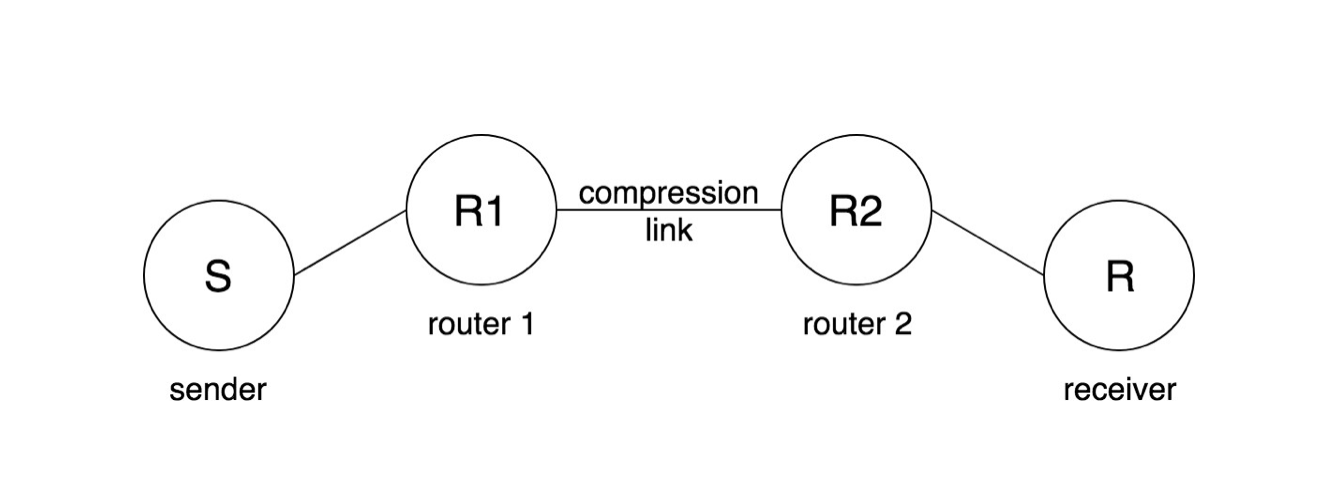
\includegraphics[width=\textwidth]{topology}
%%  \caption{5-nodes topology implemented}
%%  \label{fig:topology}
%% \end{teaserfigure}

%%
%% This command processes the author and affiliation and title
%% information and builds the first part of the formatted document.
\maketitle

\section{Introduction}
Historically, data compression \cite{lelewer1987data} topic has been in the research and the industry field for the past decades and attracted significant attention due to its efficiency capability on in the data transmission and storage. It has been widely used to minimize disk utilization, decrease bandwidth consumption on the networks and reduces energy consumption in the hardware \cite{welton2011improving}
In the recent research work and in the field of the data transmission and networking area, Shimamura et al. (2010) proposed a compression strategy meant to reduce the packages lost between the network based on the hypothesis that the advanced relay nodes are located inside the network, and they have computational, storage and network resources nodes\cite{shimamura2010compressing}. 

In 2013,  Songbin Liu et al. proposed a versatile compression method for floating point data. They claimed their design can achieve much better compression ratios than existing general purpose compression methods with promising throughputs and it can support a asymmetric decompression. \cite{liu2013versatile} 

Later, in 2016 Shamieh et al. \cite{shamieh2016adaptive} introduced  an adaptive and distributed compression/decompression scheme. The new adaptive scheme was needed because of the unexpected growth of the traffic which triggered a set of incentive/challenges such as: high congestion in the networks, high loss rates of the packets and latency. The previous mentioned challenges had a higher impact over the performance of the network and in the same time had a negative impact on Quality of Service (QoS) . The author suggested an adaptive and distributed compression/decompression model for reducing the congestion in the network and at the same time support/maintain the QoS.

Dong Tian (2017) found the geometry distortion of point cloud measurement  a challenging task and proposed using point to plane distances as measure of geometric distortions on point cloud compression. the intrinsic resolution of the point clouds was proposed as a normalizer to convert the mean square error to PSNR numbers. \cite{tian2017geometric}

Although there is a lot of work related to compressing and sending data through a network \cite{serfozo1999little}\cite{shimamura2010compressing}\cite{tan2010enhanced} this become day by day a complex and a challenging topic as a result of traffic growth. 
Hence, in this proposed research work the effort is taken to design and implement the embedded external compression library in a compression line capacity and analyze the behavior of data travelling when they placed in the bottle-neck of capacity link. 

\section{Design }
High speed application become considerable especially when there is a high traffic in the network. In order to generate high traffic, a single topology 
with 5 nodes was designed and implemented using point to point protocol standard library in the NS-3 environment. Figure ~\ref{fig:Topo} shows the topology designed in this project. 
The middle link was used to generate bottleneck link. First node and the last 
node act as client and server application where the sender sends two sets of 
6000 user data-gram protocol (UDP) packets back-to-back as packet train, and the receiver records the 
arrival time between the first and last packet in the train. The first packet train 
consists of all  of size 1100 bytes in payload, filled with all zeros, while the 
second packet train contains random sequence of bits. This configuration generates high traffic in the middle point to point link that makes it suitable environment to implement data compression on the top of the application.
 

\subsection{Data Compression}

 In order to fully utilize the network path especially in the bottleneck of the network data compression is introduced. In this project zLib external library was implemented to compress data in pre-link path. zlib \cite{Deutsch:1996:ZCD:RFC1950} is a software library used for data compression 
 and is an abstraction of the DEFLATE compression algorithm used in their gzip file compression program. The zlib library is also a crucial component of many software platform as the compressed data format is itself portable across platforms.
The compression link application was embedded and built using NS-3. 
The implemented Lempel-Ziv-Stac \cite{Deutsch:1996:ZCD:RFC1950} compression algorithm is  responsible for 
compression and decompression of incoming and outgoing packets and follows 
RFC 1974 PPP Stac LZS Compression Protocol \cite{Deutsch:1996:ZCD:RFC1950} requirement.
For the purposes of this project, the entire packets are inspected upon the arrival for checking the protocol number.  Matched protocol packet then is pushed for compression process. The pre-processing  finds the matched packet to replace the original protocol number with the LZS protocol number, 0x4021. 

\begin{figure}[h]
  \centering
  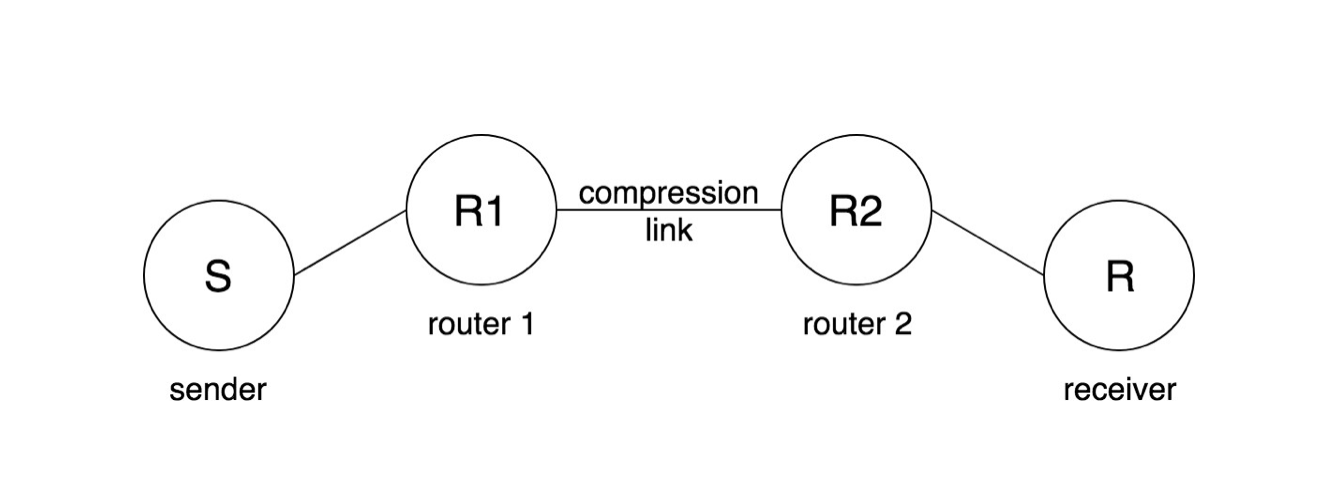
\includegraphics[width=\linewidth]{topology}
  \caption{Designed 5 nodes topology with point-to-point compression link }
  \label{fig:Topo}
\end{figure}

Original protocol number is appended to the original data, and compress that whole bit-string and replace it with the original data section in the original packet, as illustrated in Figure ~\ref{fig:Topo}. 
In the other hand, decompression, at the other side of the compression link then reverses all the pre-processing steps performed at the compression, to retrieve the original incoming packet, before pushing it to the next interface. The assumption is the two routers have already reached an Opened state and LZS has been negotiated as the primary compression algorithm. Similarly, there is no implementation from the negotiation phase specified in X3.241-1994. The compression and decompression algorithm is implemented in PointToPointNetDevice to enable compression/decompression on the point-to-point links in NS-3 environment. 

\begin{figure}[h]
  \centering
  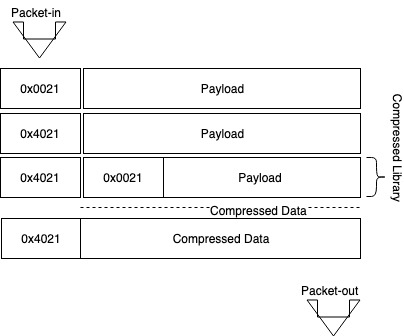
\includegraphics[width=\linewidth]{compression}
  \caption{The specified method to implement for assembling compressed packets, as specified in RFC 1974\cite{Deutsch:1996:ZCD:RFC1950}}
  \label{comp}
\end{figure}

The higher level of compression and decompression implementation model is shown in Figure ~\ref{comp}.
\subsection{Compression Detection Algorithm}
The network compression detection is implemented only in the cooperative environment as described. The proposed network application is implemented as a client/server application where the sender sends two sets of 6000 UDP packets as packet train one zero payload and the other random generated payload. The random sequence generator is implemented using /dev/random library in Linux. In order to detect compression, a threshold value is introduced. Although, there is no threshold for success for compression detection and the compression classification has never been attempted as a machine learning problem \cite{hahn2018detecting}, based on our research criteria we have select 100 ms threshold for the compression detection .  If the difference in arrival time between the first and last packets of the two trains is more than a fixed threshold of 100 ms, the application reports compression detection event, whereas when the time difference is less than 100 there was probably no compression link on the path and the application will report no compression event was detected. 

\begin{displaymath}
	\Delta tH_{HighEntropy}  = T_{FirstPktArrival} - T_{LastPktArrival} 
\end{displaymath}
\begin{displaymath}
	\Delta tL_{LowEntropy}  = T_{FirstPktArrival} - T_{LastPktArrival} 
\end{displaymath}
\begin{equation}
 	DetectionFactor = \Delta tH - \Delta tL
\end{equation}
\label{delta}


The proposed compression algorithm is configured with one command-line argument, Compression Link Capacity, which specifies the maximum bandwidth across the link between the two routers. compression link capacity is tuned to find the compression efficiency. The implementation of add-on feature in SEND() packet model in the ns-3 library is shown here:

 \begin{lstlisting}
/*
* Compression Model Implementation
*/
 if(this -> doCompress){   
    PppHeader header;
    packet-> RemoveHeader(header);
    if(header.GetProtocol()==this->compressProtocolNumber){      
    /* Remove IPV4 Header */
    Ipv4Header ipHeader;
    packet-> RemoveHeader(ipHeader);
    /* Remove UDP Header */
    UdpHeader udpHeader;
    packet-> RemoveHeader(udpHeader);
    /* Add Data & protocol and copy to inData */
    int protocolSize = 2;
    int dataSize = packet-> GetSize();
    uLongf size = dataSize + protocolSize; 
    uint8_t *inData = new uint8_t[size];
    inData[0]=0x00; 
    inData[1]=0x21;
    packet-> CopyData(&(inData[2]),size);
    uint8_t *compressData = new uint8_t[size];
    uLongf new_size;
    int returnValue = compress2((uint8_t*)compressData, &new_size, (uint8_t*)inData  (uLongf)size,Z_BEST_COMPRESSION);     
    size = new_size;
    packet = new Packet(compressData,size); 
    size = size + 8; 
    udpHeader.ForcePayloadSize(size);
    packet-> AddHeader(udpHeader);
    ipHeader.SetPayloadSize(size); 
    packet-> AddHeader(ipHeader);
    header.SetProtocol(COMPRESSED_PROTOCOL_NUMBER); 
    } 
    packet->AddHeader(header);
  } 

\end{lstlisting}

\section{System Implementation and Verification}
As discussed earlier, the network topology was implemented in the Point-to-Point Protocol (PPP , RFC 1661) \cite{point1991autonet} model library. The native PPP link is assumed to be established and authenticated at all the time. 
\begin{figure}[h]
  \centering
  \includegraphics[width=\linewidth]{topoImp}
  \caption{Five nodes topology}
  \label{topoImp}
\end{figure}

The proposed project was run under a 5-node topology in NS-3 environment as shown in Figure ~\ref{fig:topoImp}. Nodes sender and receiver are the end-hosts running the network application. Nodes R1 and R2 are the intermediate routers where the link between them is compression-enabled. The project topology was built under NS-3 environment using point to point link library. It includes four logically separate simulations, each doing one of the following: 
\begin{itemize}
\item Transmit low entropy data over a network topology without a compression link.
\item Transmit high entropy data over a network topology without a compression link. 
\item Transmit low entropy data over a network topology with a compression link. 
\item Transmit high entropy data over a network topology with a compression link.
\end{itemize}

The control for confounding variables across the the simulations were defined precisely, as it ultimately be comparing time between the  simulation types to detect the compression link. The whole system is automated to run the first low entropy packet train followed by the high entropy packet train. 
The middle capacity link (router A, router B) then varies and tuned with different capacity parameter from 1 to 10 Mbps, reporting each $\Delta$tH - $\Delta$tL . The link capacity of the two outer (non compression) links on the four node topology was set persistently to 5 Mbps. Proposed two senders in the topology supports low and high entropy respectively. Sender and receiver nodes are UDP server and clients. Receiver nodes records the arrival time between the first and last packet in the simulation. There are three main components designed and implemented in this architecture.

\begin{itemize}
\item Configuration Management System
\item Topology Management System
\item Compression System
\item Synchronization and Output Recorder
\end{itemize}

protocol check, payload management, compression and decompression feature were hosted in the point-to-point-net-device class library. The UDP-client model class were modified to generate random payload in high entropy traffic and UDP-server model class host the entire calculation and compression detection algorithm. The external zLib \cite{Deutsch:1996:ZCD:RFC1950} - An abstract of the DEFLATE compression algorithm - was embed with project to perform compression task and as such output data length of compression link varied due to compression process.  
In order to build the project ./waf build system was implemented. the following command build the project while compression system is enabled. 
 
 \begin{lstlisting}
/*
* To compile and build the project
*/
 $ cd workspace/Transport-Layer-Security/ns-3-allinone/ns-3-dev    
 $ ./waf configure
 $ ./waf build
 $ ./waf --run "scratch/point2point --IsHighEntropy=1 --IsCompress=1 --MaxPacketCount=2"

\end{lstlisting}

In the topology management, two UDP client and an UDP server and point to point net devices were initiated. The Initialized class implementation is shown for low entropy UDP Client. The device attribute for the link between router 1 and router 2 was set for data rate, delay and maximum transmit unit (MTU). The compression and decompression flag was set while initializing the topology. The point to point net device library was modified to support the following features: 
 
\begin{itemize}
\item Protocol Checker
\item Payload Management
\item Compression and Decompression
\end{itemize}
 
 SEND method in point to point net device host compression design while RECEIVE method host Decompression design. The arriving PPP packets were parse to capture protocol and if protocol number matched with configuration management system. If checked packet type matches one in the configuration file, the payload will be taken and compressed based on zLib library. and the protocol will be replaced with LZS protocol number. and the newly generated packet will be sent to Decompression router through the link.  
In the other hand, RECEIVE function decompressed the packet payload data after removing all necessary header file.   
 
 \begin{figure}[h]
  \centering
  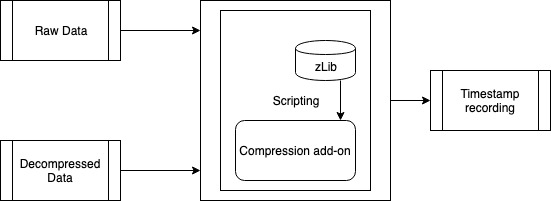
\includegraphics[width=\linewidth]{zlib}
  \caption{Embedded add-on zlib library }
  \label{zlib}
\end{figure} 

The designed system is smart to detect and to target only compressed packet for decompression process. Figure \ref{zlib} shows the header file involved with the arriving packet and the compression process on the packet. 
Second UDP client is in-charge to generate high entropy trained packet and run it through the network. 

\begin{equation}
 	DetectionFactor = \Delta tH - \Delta tL \label{eq:2}
\end{equation}


The same process will take place for high entropy trained packet. In the other hand, UDP server counts the incoming packets and calculates the delta high entropy and the delta low entropy based on the equation \ref{eq:2}.\\
To detect the compression threshold value of 100 ms was defined.  The delta time difference more than the threshold value triggers the detection flag and vice a versa. Timing report of the delta is logged and store in the repository.  
 
Client and server application where the senders send 6000 UDP packets and the receiver records the arrival time between the first and the last packet in the train . the first packet train consists of all packets of size 1100 bytes in their payload, filled with zeros while the second packet trains contains random sequence of bits. If the difference in arrival time between the first and last packets of the two trains is more than the fixed threshold of 100 ms, the application reports compression detected whilst when the time difference is less than the threshold value, there is probably no compression link in the path and the application reports no compression is detected. The middle link data rate was modified within the range of 1 Mbps up to 10 Mbps to generate bottleneck of data on the link. 

 \begin{figure}[h]
  \centering
  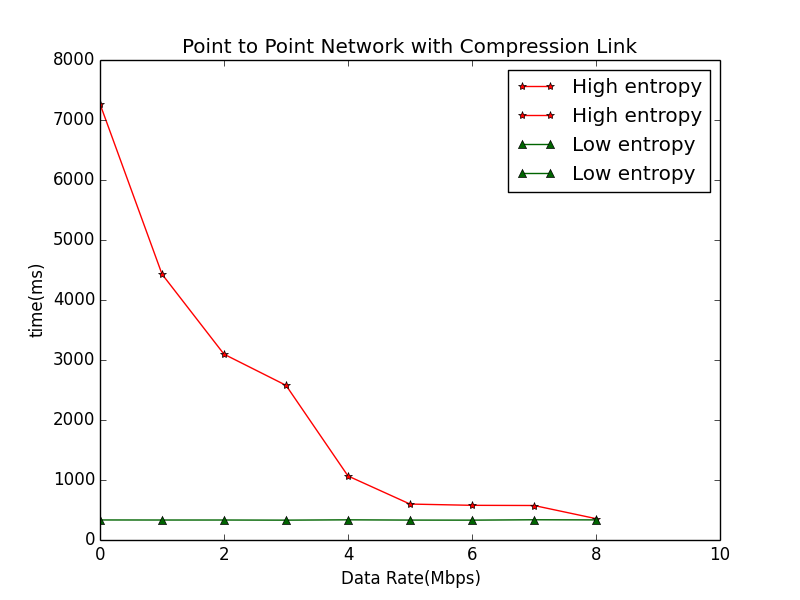
\includegraphics[width=\linewidth]{timing}
  \caption{High and low entropy train on the server node arrival time }
  \label{t1}
\end{figure} 

Figure \ref{t1} shows the timing reported on link capacity with low entropy packet train and high entropy packet train while two outer link on the node topology was set to 8 Mbps consistently. The compression capacity link was varied to realize the compression behavior in different data rate configuration. 

 \begin{figure}[h]
  \centering
  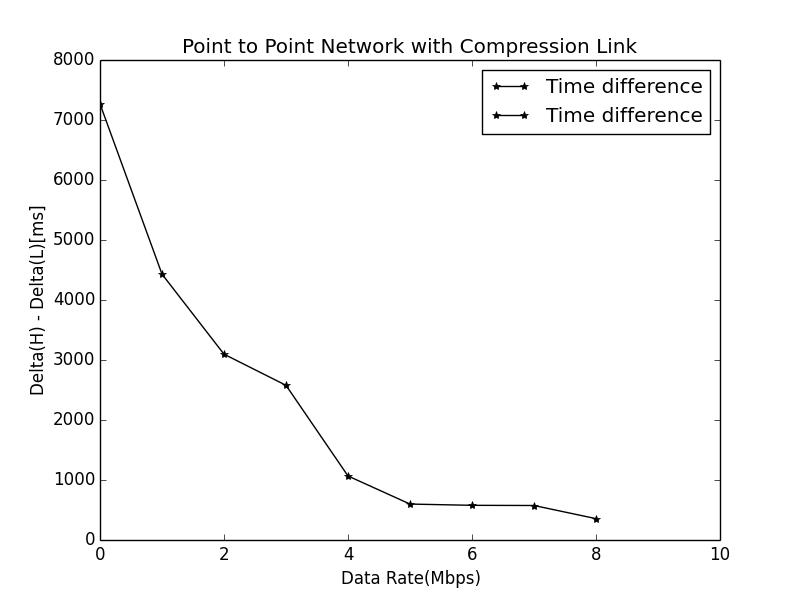
\includegraphics[width=\linewidth]{timing2}
  \caption{Arrival time difference between high and low entropy packet train on the server node }
  \label{t2}
\end{figure} 

The time difference between high and low entropy packet train was shown in Figure \ref{t2} . While network bandwidth is steadily increasing, the arrival time of low entropy packet train does not show much timing difference in compression link while there is significant behavior change is observed when high entropy packet train is located in the high bandwidth capacity link that shows the compression affect in the bottle-neck of the capacity link. 

\section{Conclusion}
This research has concentrated on design and implementation of  embedded efficient compression and fast decompression model to enhance data transferring speed in the network traffic. The external zlib library was embed with the designed topology to perform compression. The packet trains with low and high entropy were generated to be transferred in compression capacity link for data evaluation and further investigation. Data analysis was performed and it was critical for analytic queries that repeatedly and synchronously read compressed packet data arrival time. The arrival time of the first packet trained and the last packet trained of each series were captured and plotted. The result shows the although data compression enhance the data transmission speed yet it is only effective the capacity link turns as bottle-neck. Compression has no effect on data transmission speed if there is no bottle-neck exists in the capacity compression link. The Compression and decompression model was added to ns-3 library as a new feature. 
%%
%% The acknowledgments section is defined using the "acks" environment
%% (and NOT an unnumbered section). This ensures the proper
%% identification of the section in the article metadata, and the
%% consistent spelling of the heading.


%%
%% The next two lines define the bibliography style to be used, and
%% the bibliography file.
\bibliographystyle{ACM-Reference-Format}
\bibliography{sample-base}

%%
%% If your work has an appendix, this is the place to put it.


\end{document}
\endinput
%%
%% End of file `sample-xelatex.tex'.
